\subsection{\textit{Frontend}}
Um dos requisitos do projeto é o desenvolvimento do \textit{frontend} com a utilização de \textit{Flutter}, visto que a empresa no seu trabalho diário já utiliza esta ferramenta. Deste modo, foi fulcral a aprendizagem desta ferramenta e da sua linguagem de programação o Dart.

\subsubsection{Desenvolvimento cross-platform}
O desenvolvimento de aplicações \textit{cross-platform} ou multi-plataforma, consiste no desenvolvimento de uma aplicação para diversas plataformas e este pode ser realizado de diversas formas, mas as principais formas conhecidas são WebView, nativo e outras abordagens.

As \emph{frameworks} nativas são "(...)\emph{the most stable choice for mobile application development}(...)"\citep{flutter} e dispõem de uma grande comunidade e leque de aplicações desenvolvidas. O que torna estas \textit{frameworks} estáveis é o facto de "(...)\emph{the app in this framework talks directly to the system}(...)"\citep{flutter}. Todo o desenho no ecrã é realizado através de o que é chamado de \emph{OEM components} que são disponibilizados pela \emph{framework} mas não permitem customização total. A grande desvantagem desta abordagem é o facto de se o objetivo do projeto é o desenvolvimento para \textit{iOS} e \textit{Android}, então "(...)\emph{you need to learn two different languages}(...)"\citep{flutter}, porque estas são utilizadas para "(...)\emph{write two different apps with the same functionalities}(...)"\citep{flutter} o que significa que "(...)\emph{every modification must be duplicated on both platforms}(...)"\citep{flutter}.

Uma outra abordagem para o desenvolvimento para diversas plataformas é através de uma única base de código como o \textit{WebView}. "(...)\emph{Cordova-, Ionic-, PhoneGap-, and WebView-based frameworks in general are good examples of cross-platform frameworks}(...)"\citep{flutter}, mas o grande problema desta abordagem é a "(...)\emph{lack in performance}(...)"\citep{flutter} pois esta é composta por um processo intermédio chamado \textit{WebView} que renderiza código \textit{HTML}, isto significa que "(...)\emph{the app is basically a website}(...)"\citep{flutter}.
Esta abordagem acrescenta também o componente de ponte que realiza o "(...)\emph{switch between JavaScript to the native system}(...)"\citep{flutter} para obter acesso aos serviços nativos.

Um concorrente à tecnologia mencionada na secção (\ref{flutter_explaining}) é o \textit{React Native}, este assim como as \textit{frameworks} nativas "(...)\emph{heavily relies on OEM components}(...)"\citep{flutter} e "(...)\emph{expands the bridge concept in the WebView systems, and uses it not only for services, but also to build widgets}(...)"\citep{flutter}, isto leva a grandes problemas em termos de performance devido a que "(...)\emph{a component may be built hundreds of times during an animation, but due to the expanded concept of the bridge, this component may slow down to a great extent}(...)"\citep{flutter}.

\subsubsection{Flutter}\label{flutter_explaining}
\textit{Flutter} é uma \textit{framework} desenvolvida pela \textit{Google}, de inicio "(...)\emph{was an experiment, as the developers at Google were trying to remove a few compatibility supports from Chrome, to try to make it run smoother}(...)"\citep{flutter}, por fim, acabaram por descobrir que "(...)\emph{they had something that rendered 20 times faster than Chrome did and saw that it had the potential to be something great}(...)"\citep{flutter}. Em suma, \textit{Google} desenvolveu "(...)\emph{a layered framework that communicated directly with the CPU and the GPU in order to allow the developer to customize the applications as much as possible}(...)"\citep{flutter}.

Para o \textit{Flutter} tudo é um \textit{widget}, "(...)\emph{Orientation, layout, opacity,animation... everything is just a widget}(...)"\citep{flutter}, isto permite que os utilizadores "(...)\emph{choose composition over inheritance, making the construction of an app as simple as building a Lego tower}(...)"\citep{flutter}. Todos estes \textit{widgets} oficiais estão identificados no catálogo de widgets do \textit{Flutter}. Como tudo no \textit{Flutter} é composto por \textit{widgets} "(...)\emph{the more you learn how to use, create, and compose them,the better and faster you become at using Flutter}(...)"\citep{flutter}.

A abordagem ao \textit{cross-platform} realizada pelo \textit{Flutter} é baseada em "(...)\emph{AOT (Ahead Of Time) instead of JIT (Just In Time) like the JavaScript solutions}(...)"\citep{flutter} mostradas anteriormente. Esta também permite a conversação direta com o cpu sem necessidade de ponte e "(...)\emph{does not rely on the OEM platform}(...)"\citep{flutter}. Esta faculta que "(...)\emph{custom components to use all the pixels in the screen}(...)"\citep{flutter}, o que significa que "(...)\emph{the app displays the same on every version of Android and iOS}(...)"\citep{flutter}. Esta também utiliza "(...)\emph{Platform Channels to use the services}(...)"\citep{flutter}, o que leva a que "(...)\emph{if you need to use a specific Android or iOS feature, you can do it easily}(...)"\citep{flutter}.
\subsubsection{Dart}
\textit{Dart} é a linguagem de programação utilizada pela \textit{framework Flutter}, esta é "(...)\emph{a general purpose programming language}(...)"\citep{dart_pg_lang} que foi desenhada para ser "(...)\emph{familiar to the vast majority of programmers}(...)"\citep{dart_pg_lang}. Esta linguagem é "(...)\emph{purely object-oriented}(...)" o que significa que "(...)\emph{all values a Dart program manipulates at run time are objects}(...)"\citep{dart_pg_lang}, até tipos básicos como números e booleanos, esta é também "(...)\emph{class-based, optionally typed}(...)"\citep{dart_pg_lang}. Esta é opcionalmente tipada, o que significa que a decisão de utilizar tipagens cai sobre o programador, mas no caso de \textit{Flutter}, na sua versão mais recente é recomendado a utilização de tipagens de variáveis. Por fim, esta "(...)\emph{supports mixin-based inheritance and actor-style concurrency}(...)"\citep{dart_pg_lang}.
\subsection{Links de aplicações}

Existem diferentes tipos de \textit{links} sendo que para \textit{mobile} é utilizado os \textit{app links}, \textit{deep links} e os \textit{dynamic links}.

Os \emph{app links} são "(...)\emph{web links that use the HTTP and HTTPS schemes}(...)"\citep{linking}, estes possuem também um atributo extra chamado \textit{autoVerify}. Este atributo permite a uma aplicação "(...)\emph{to designate itself as the default handler of a given type of link}(...)"\citep{linking}, isto permite que "(...)\emph{app opens immediately if it's installed}(...)"\citep{linking}. O grande problema é que estes \textit{links} não permitem o redirecionamento do utilizador para uma parte específica da aplicação e é necessário dispor de um domínio próprio.


Os \textit{deep links} são "(...)\emph{URIs of any scheme that take users directly to a specific part of your app}(...)"\citep{linking}, o grande problema deste tipo de \textit{links} é que se os utilizadores não dispuserem da aplicação instalada no dispositivo, este irá falhar e não permite a customização de comportamento.

Já os \textit{dynamic links}, desenvolvidos pela \textit{Firebase}, assim como os \textit{deep links} "(...)\emph{if a user opens a Dynamic Link on iOS or Android, they can be taken directly to the linked content in your native app}(...)"\citep{dynamic_linking}, mas para além disto, este permite que "(...)\emph{if a user opens the same Dynamic Link in a desktop browser, they can be taken to the equivalent content on your website}(...)"\citep{dynamic_linking}, ou seja, este permite a customização de comportamento de \textit{links} para diversas situações e em caso do utilizador não dispor da aplicação instalada, este permite que "(...)\emph{the user can be prompted to install it; then, after installation, your app starts and can access the link}(...)"\citep{dynamic_linking}. Visto que este é o comportamento desejado pelo cliente da aplicação, então foi decidido utilizar esta abordagem.

\begin{figure}[htb]
  \centering
  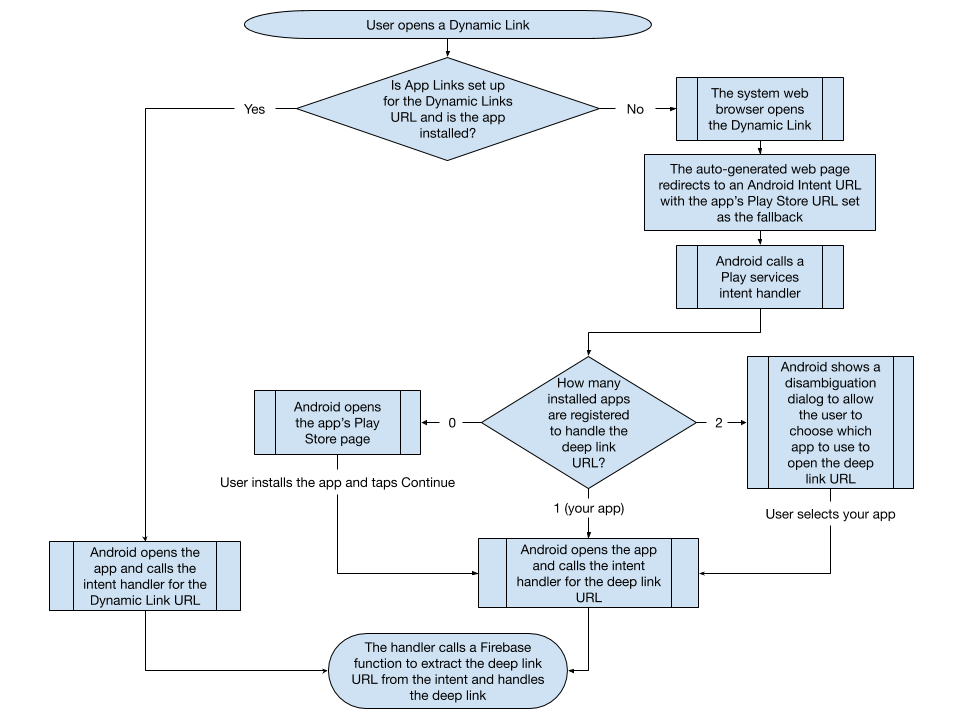
\includegraphics[width=0.83\textwidth]{images/diagramas/fdl-android-integration.png}
  \caption{Funcionamento dos dynamic links \citep{linking_firebase}}
  \label{fig:23}
\end{figure}


